\documentclass[12pt, a4paper]{article}

% Configuración de márgenes de las páginas
	\usepackage{a4wide}

% Paquete de acentos para Linux
	\usepackage[utf8]{inputenc}

% Paquete para reconocer la separación en sílabas en español
	\usepackage[spanish]{babel}

% Paquetes especiales para el TP
	\usepackage{caratula}

%	Paquete para simbolos matemáticos
	\usepackage{amssymb}			
	\usepackage{amsmath}

% Paquete para armar índices
	\usepackage{makeidx}
	\makeindex

% Más espacio entre líneas
	\parskip=1.5pt

% Otros paquetes
	\usepackage{graphicx}
	\usepackage{float}
	\usepackage{listings}
	\usepackage{color}
	\usepackage{url}
	\definecolor{lnk}{rgb}{0,0,0.4}
	\usepackage[colorlinks=true,linkcolor=lnk,citecolor=blue,urlcolor=blue]{hyperref}
	\usepackage{wrapfig}

% Importo los comandos personalizados
	\newcommand{\func}[2]{\texttt{#1}(#2) :}
\newcommand{\tab}{\hspace*{2em}}
\newcommand{\FOR}{\textbf{for }}
\newcommand{\TO}{\textbf{ to }}
\newcommand{\IF}{\textbf{if }}
\newcommand{\WHILE}{\textbf{while }}
\newcommand{\THEN}{\textbf{then }}
\newcommand{\ELSE}{\textbf{else }}
\newcommand{\RET}{\textbf{return }}
\newcommand{\MOD}{\textbf{ \% }}
\newcommand{\OR}{\textbf{ or }}
\newcommand{\NOT}{\textbf{ not }}
\newcommand{\tOde}[1]{\tab \small{\mathcal{O}($#1$)}}
\newcommand{\Ode}[1]{\ensuremath{\small{\mathcal{O}\left(#1\right)}}}
\newcommand{\VSP}{\vspace*{3em}}
\newcommand{\Pa}{\vspace{5mm}}
\newcommand{\iif}{\Leftrightarrow}
\newcommand{\gra}[1]{\noindent\includegraphics[scale=.70]{#1}\\}
\newcommand{\gras}[2]{\noindent\includegraphics[scale=#2]{#1}\\}
\newcommand{\gram}[1]{\noindent\includegraphics[scale=.50]{#1}}
\newcommand{\dirmail}[1]{\normalsize{\texttt{#1}}}
\newcommand{\superref}[1]{\textsuperscript{\ref{#1}}}

\newenvironment{pseudo}{\noindent\begin{tabular}{ll}}{\end{tabular}\VSP}
\newenvironment{while}{\WHILE \\ \setlength{\leftmargin}{0em} }{}
\newenvironment{usection}[1]{\newpage\begin{section}*{#1}	\addcontentsline{toc}{section}{#1}}{\end{section}}
\newenvironment{usubsection}[1]{\begin{subsection}*{#1}	\addcontentsline{toc}{subsection}{#1}}{\end{subsection}}


	\lstset{language=C,basicstyle=\small\tt,keywordstyle=\bf,tabsize=3,breaklines=true,linewidth=16cm,postbreak={\mbox{$\rightsquigarrow$}},prebreak={\mbox{$\rightsquigarrow$}}}


\begin{document}

% Carátula
	\titulo{Trabajo Práctico Nº1}
	\fecha{12 de Octubre de 2010}
	\materia{Sistemas Complejos en Máquinas Paralelas}
	\grupo{  }
	\integrante{Allekotte, Kevin}{490/08}{kevinalle@gmail.com}
	\maketitle

	\newpage		\printindex \tableofcontents
	
	\section{Discretización del Sistema}
		Queremos resolver por el método de \textit{Diferencias Finitas} la ecuación transitoria de calor en 1D usando el método alfa para la discretización temporal.
		
		La ecuacion es:
		$$\frac{\partial u}{\partial t}=K\frac{\partial^2 u}{\partial x^2}$$
		
		\subsection{Adimensionalización del Sistema}
			Planteamos la ecuación para $x'$ y $t'$ con:
			$$x'=\frac{x}{x_0} \qquad t'=\frac{t}{t_0}$$
			
			Y obtenemos como resultado
			$$\frac{\partial u}{\partial (t' t_0)}=K\frac{\partial^2 u}{\partial (x' x_0)^2}$$
			
			Entonces el sistema adimensionalizado es
			$$\frac{\partial u}{\partial t'}=\left(\frac{t_0 K}{x_0^2}\right)\frac{\partial^2 u}{\partial x'^2}=K'\frac{\partial^2 u}{\partial x'^2}$$
		
		\subsection{Discretización}
			$$u(x,t) \longrightarrow u(x_i,t_n)=\mathbf{u}_{i,n}$$
			
			\subsubsection{Condiciones Iniciales y de Borde}
				$$\mathbf{u}_i^0=F(i) \qquad \mathbf{u}_0^n=\text{Condicion de borde Izquierdo} \qquad \mathbf{u}_1^n=\text{Condicion de borde Derecho}$$
			
			\subsubsection{$\alpha=0$}
				$$\frac{\mathbf{u}_i^{n+1}-\mathbf{u}_i^n}{k}=K'\frac{\mathbf{u}_{i+1}^n-2\mathbf{u}_i^n+\mathbf{u}_{i-1}^n}{h^2}$$
				$$\mathbf{u}_i^{n+1}=r\mathbf{u}_{i+1}^n+(1-2r)\mathbf{u}_i^n+r\mathbf{u}_{i-1}^n \qquad r=\frac{kK'}{h^2}$$

			\subsubsection{$\alpha=1$}
				$$\frac{\mathbf{u}_i^{n+1}-\mathbf{u}_i^n}{k}=K'\frac{\mathbf{u}_{i+1}^{n+1}-2\mathbf{u}_i^{n+1}+\mathbf{u}_{i-1}^{n+1}}{h^2}$$
				$$\mathbf{u}_i^{n+1}=\frac{r}{1+2r}(\mathbf{u}_{i+1}^{n+1}+\mathbf{u}_{i-1}^{n+1}) + \frac{\mathbf{u}_i^n}{1+2r}$$
	
	\section{Resolución Numérica Serial}		
		\subsection{$\alpha=0$}
			Para resolver el sistema con $\alpha=0$ se puede hacer un vector y para cada intervalo de tiempo se cambia el valor de $\mathbf{u}_i$ por $r\mathbf{u}_{i+1}+(1-2r)\mathbf{u}_i+r\mathbf{u}_{i-1}$.
		
			\subsubsection{Código}
				\lstinputlisting{../difusion.cpp}
			
			\subsubsection{Resultado}
				\begin{center}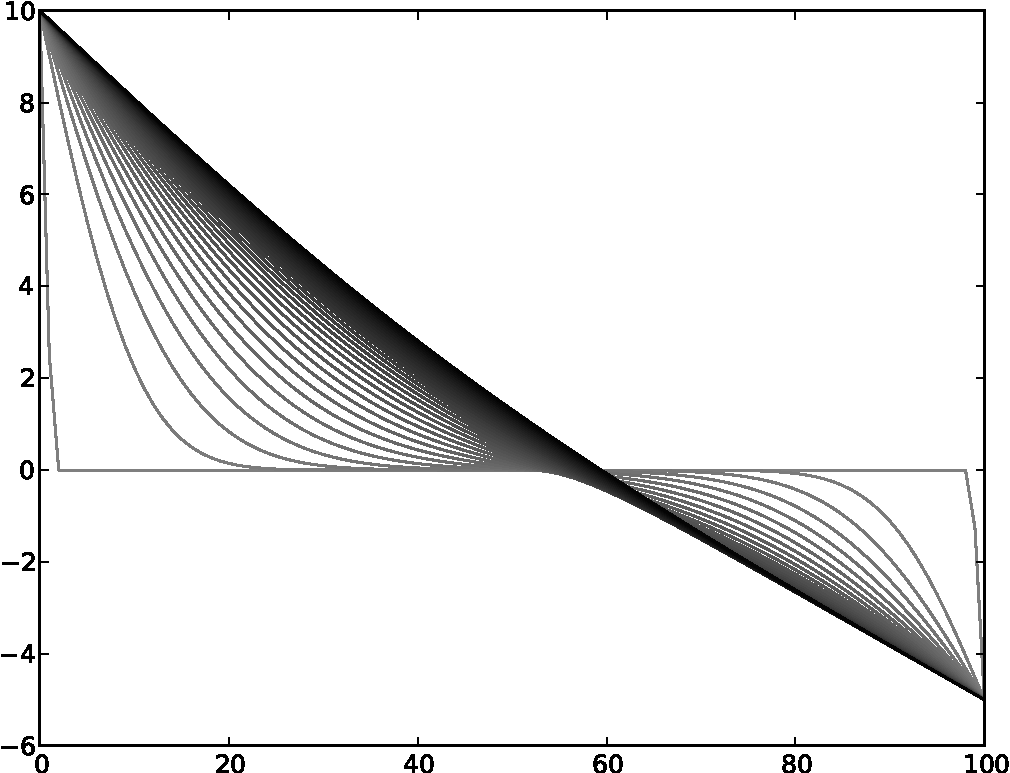
\includegraphics[width=.9\textwidth]{alpha0.pdf}\end{center}
				
				Las líneas más oscuras representan el estado a mayor tiempo.
				
				El resultado es el esperado :)
		
		\subsection{$\alpha=1$}
			Con $\alpha=1$ el programa es muy parecido, pero en vez de usar el valor de la iteración anterior, se usa el de la iteración actual.
			Para eso en necesario usar la técnica de Gauss-Seidel que converge a la solución.
			
			\subsubsection{Código}
				La única parte relevante del código es la siguiente:
\begin{lstlisting}
forn(iter,20){
	forsn(i,1,samples-1){
		u2[i]=(r/(1+2*r))*(u2[i+1]+u2[i-1])+u[i]/(1+2*r);
	}
}
\end{lstlisting}
				
				(Observar que la cantidad de iteriaciones está fija y no se chequea la convergencia)
			
			\subsubsection{Resultado}
				\begin{center}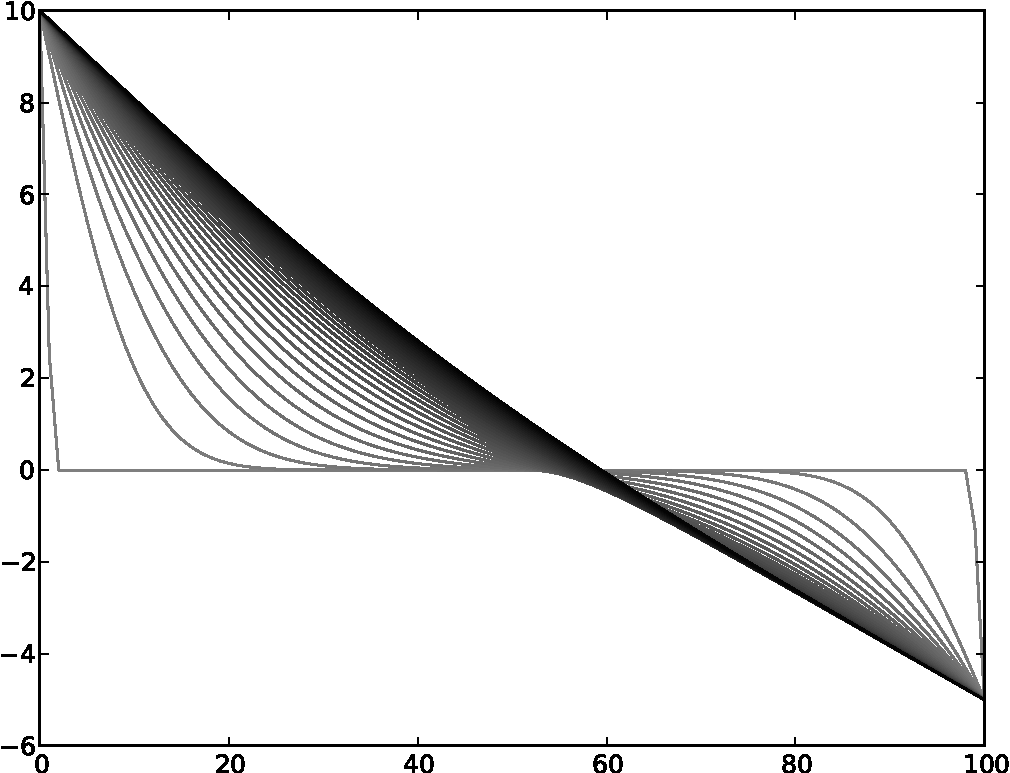
\includegraphics[width=.9\textwidth]{alpha0.pdf}\end{center}
				Nuevamente el resultado es el esperado.
		
		\section{Condiciones Iniciales y de Borde}
			$$F(x)=\begin{cases}10 & 0<x\leq 0.5\\ -5 & 0.5<x<1\end{cases}$$
			\begin{center}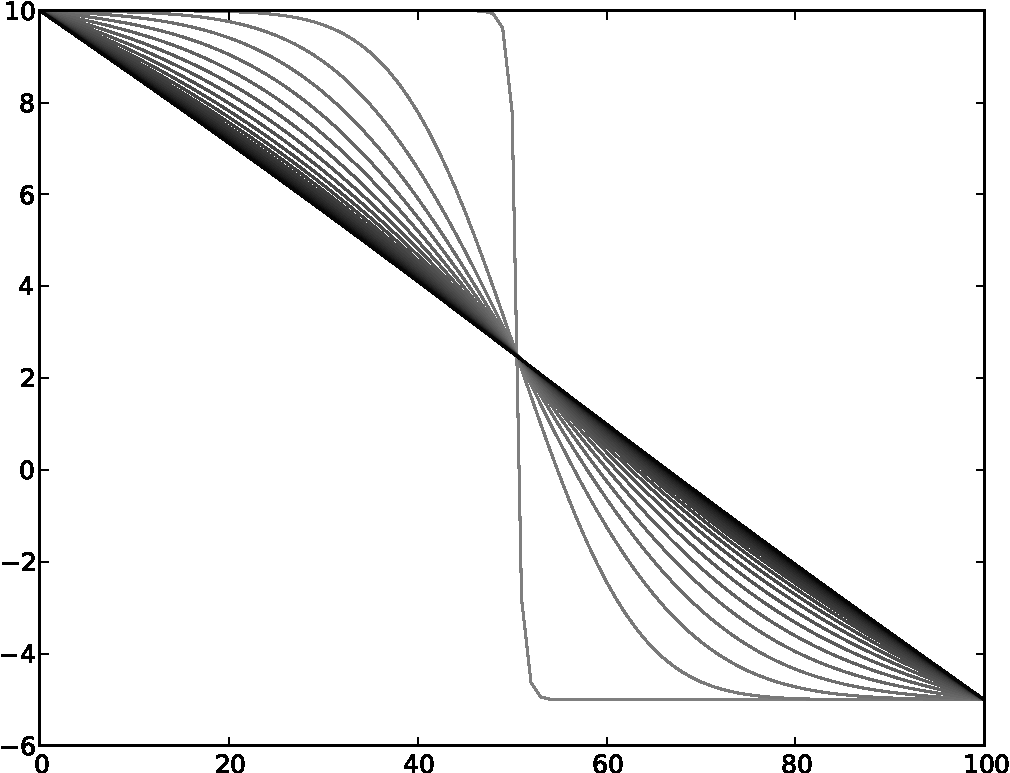
\includegraphics[width=.8\textwidth]{3a.pdf}\end{center}
			
			$$\mathbf{u}_0 = 5cos(100t)$$
			\begin{center}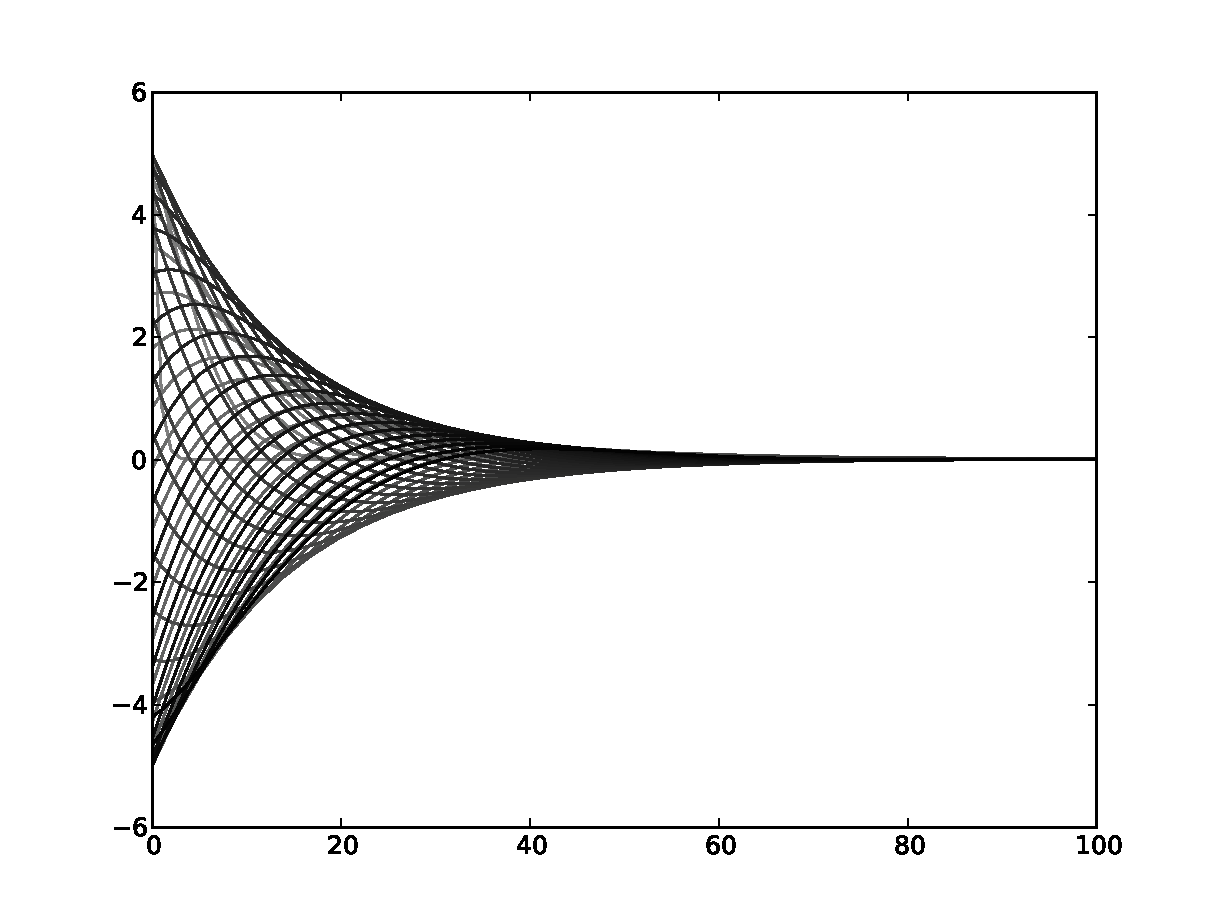
\includegraphics[width=.8\textwidth]{3b.pdf}\end{center}
		
		\section{Implementación en paralelo: \texttt{MPI}}
			Procedemos a implementar la solución en una máquina paralela.
			La idea es dividir el vector en porciones aproximadamente iguales, y resolver cada pedazo en un core.
			
			Utilizamos la librería \texttt{MPI} que nos brinda operaciones de ejecución en paralelo y comunicación entre los procesos.
			El proceso root (0) no va a hacer cálculos sino que va a coordinar a los otros procesos, recibir los resultados, y comunicarse con el usuario.
			
			Una vez dividido el vector, cada core ejecuta una algoritmo muy parecido al anterior, pero ahora tenemos el problema de los nodos compartidos.
			Los procesos vecinos van a necesitar información del borde del adyacente.
			Esto se puede resolver con envío de mensajes sincrónicos (bloqueantes).
			Antes de cada iteración, los procesos envían y reciben la información necesaria de sus vecinos.
			
			Cuando tienen resultados, éstos son enviados al root para que imprima la salida.
			
			\subsection{Código}
				\lstinputlisting{../difusion_mpi.cpp}
			
			\subsection{Resultado}
				Nuevamente, los resultados son los mismos que el programa en serie
				\begin{center}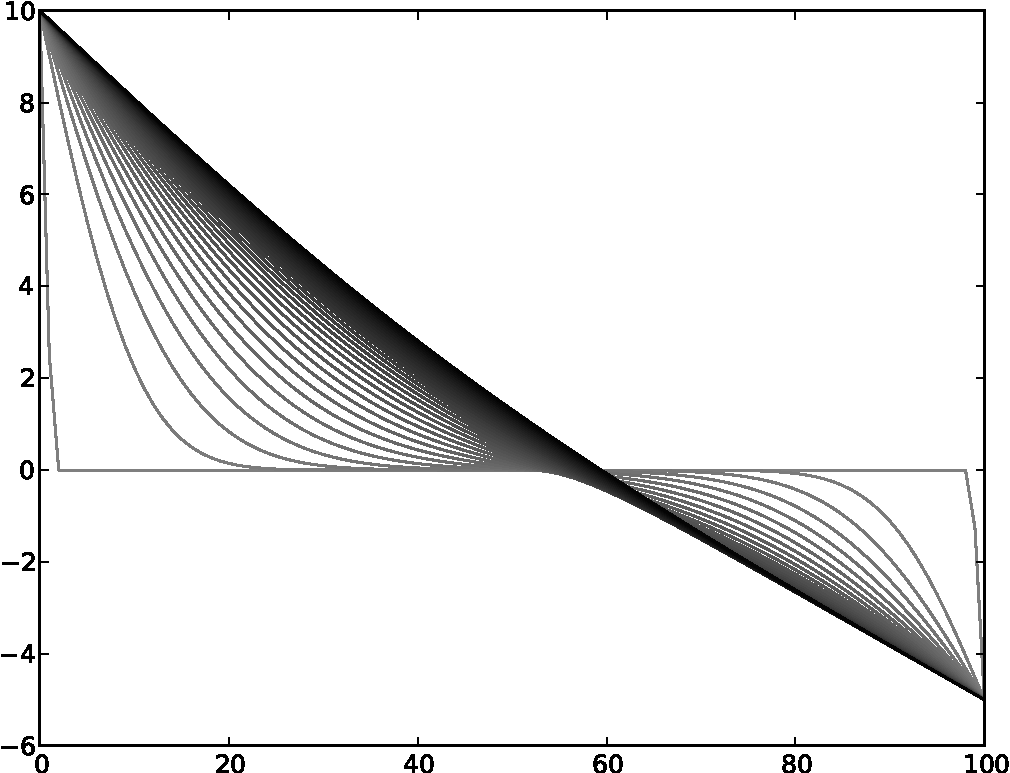
\includegraphics[width=.9\textwidth]{alpha0.pdf}\end{center}
		
		\section{Compilación y ejecución}
			Los programas seriales se compilan con \texttt{g++} y se corren directamente (sin parámetros ni entrada, los valores están hardcodeados).
			Ejemplo: \texttt{g++ difusion.cpp -o difusion \&\& ./difusion}
			
			El programa con \texttt{MPI} tiene que ser compilado y ejecutado con \texttt{MPI}.
			Ejemplo: \texttt{mpiCC difusion\_mpi.cpp -o mpi \&\& mpiexec -np 5 mpi}
			
			Todas las salidas son por \texttt{stdout}
			
			Además hay un script hecho en python para visualizar los resultados que usa la librería \texttt{matplotlib}.
			Ejemplo: \texttt{./difusion | ./draw.py}\\
			\texttt{mpiexec -np 5 mpi | ./draw.py}
		
		\section{To-Do}
			Cosas que quedaron por hacer:
			\begin{itemize}
				\item Medir los tiempos de ejecución y la performance del programa paralelo.
				\item Modificar los programas para que acepten los valores seleccionados por el usuario en la línea de comandos
				\item No está implementado el caso $\alpha=0.5$
				\item El programa paralelo usa un nodo fantasma. Hay que modificarlo para que pueda usar 2,5, y 10 nodos fantasma.
			\end{itemize}
\end{document}

